\onecolumn
\chapter{Auswertung}
% Liste der genutzten Formeln für die Fehlerrechnung
\section*{Fehlerrechnung}
Für die statistische Auswertung von $n$ Messwerten $x_i$ werden folgende Größen definiert \cite{errorSkript25}:
\begin{align}
    \bar{x} &= \frac{1}{n} \sum_{i=1}^{n} x_i \vphantom{\sqrt{\sum_i^n}^2} && \text{\textcolor{gray}{Arithmetisches Mittel}} \label{eq:arithmetisches_mittel} \\
    \sigma^2 &= \frac{1}{n-1} \sum_{i=1}^{n} (x_i - \bar{x})^2 \vphantom{\sqrt{\sum_i^n}^2} && \text{\textcolor{gray}{Varianz}} \label{eq:variation} \\
    \sigma &= \sqrt{\frac{1}{n-1} \sum_{i=1}^{n} (x_i - \bar{x})^2} \vphantom{\sqrt{\sum_i^n}^2} && \text{\textcolor{gray}{Standardabweichung}} \label{eq:standardabweichung} \\
    \Delta \bar{x} &= \frac{\sigma}{\sqrt{n}} = \sqrt{\frac{1}{n(n-1)} \sum_{i=1}^n(\bar x - x_i)^2} \vphantom{\sqrt{\sum_i^n}^2} && \text{\textcolor{gray}{Fehler des Mittelwerts}} \label{eq:fehler_mittelwert} \\
    \Delta f &= \sqrt{\left(\frac{\partial f}{\partial x} \Delta x\right)^2 + \left(\frac{\partial f}{\partial y} \Delta y\right)^2} \vphantom{\sqrt{\sum_i^n}^2} && \text{\textcolor{gray}{Gauß'sches Fehlerfortpflanzungsgesetz für $f(x,y)$}} \label{eq:gauss_fehlfortpflanzung} \\
    \Delta f &= \sqrt{(\Delta x)^2 + (\Delta y)^2} \vphantom{\sqrt{\sum_i^n}^2} && \text{\textcolor{gray}{Fehler für $f = x + y$}} \label{eq:fehler_summe} \\
    \Delta f &= |a| \Delta x \vphantom{\sqrt{\sum_i^n}^2} && \text{\textcolor{gray}{Fehler für $f = ax$}} \label{eq:fehler_proportional} \\
    \frac{\Delta f}{|f|} &= \sqrt{\left(\frac{\Delta x}{x}\right)^2 + \left(\frac{\Delta y}{y}\right)^2} \vphantom{\sqrt{\sum_i^n}^2} && \text{\textcolor{gray}{relativer Fehler für $f = xy$ oder $f = x/y$}} \label{eq:relativer_fehler} \\
    \sigma &= \frac{|a_{lit} - a_{gem}|}{\sqrt{\Delta a_{lit}^2 + \Delta a_{gem}^2}} \vphantom{\sqrt{\sum_i^n}^2} && \text{\textcolor{gray}{Berechnung der signifikanten Abweichung}} \label{eq:signifikante_abweichung}
\end{align}

\twocolumn

\section{Eichung des Gasthermometers}
Wir beginnen mit der Eichung des Gasthermometers. Hierfür nutzen wir Tabelle 1 des \hyperref[Protokoll]{Protokolls}:

\begin{table}[h!]
    \centering
    \caption{Vergleich von Zwei- und Vierleiter}
    \label{tab:zweileiter_vierleiter}
    \begin{tabular}{l | c | c}
        & \textbf{Zweileiter} & \textbf{Vierleiter} \\
        \hline
        Spannung & $100,5\,\text{mV}$ & $100,1\,\text{mV}$ \\
        \hline
        Wasserdruck & $916\,\text{mBar}$ & $916\,\text{mBar}$ \\
        \hline
        \parbox{2.5cm}{Pyrometer-\\temperatur} & $-0,5^\circ\text{C}$ & $-0,6^\circ\text{C}$ \\
        \hline
        \parbox{2.5cm}{Flüssigkeits-\\temperatur} & $0,5^\circ\text{C}$ & $0,5^\circ\text{C}$
    \end{tabular}
\end{table}

Außerdem ist dem Protokoll ein Luftdruck von $1007 \, hPa$ bei $25,1^\circ C$ zu entnehmen. Dieser Druck entspricht in der \hyperref[fig:graphisch_temp_druck]{Abbildung zur Eichung des Gasthermometers} dem Punkt bei $0 \, ^\circ C$.
Dies ist unser erster Eichpunkt. Den zweiten bestimmen wir über eine Gleichung zur Normierung des Siededrucks von Wasser \cite{skript25}:
\begin{equation}
    p_{NB} = \frac{1013,5\,\text{hPa}}{p_{LD}} \cdot p_{gem}
    \label{eq:normal_siedepunkt}
\end{equation}
In dieser Gleichung steht $p_{gem}$ für den gemessenen Wasserdruck bei Siedetemperatur, $p_{LD}$ für den Luftdruck und $p_{NB}$ für den auf Normalbedingungen umgerechneten Druck, da der Siedepunkt druckabhängig ist.
Benutzen wir also die Gleichung für die \hyperref[fig:graphisch_temp_druck]{Normalbedingung}, so erhalten wir:
\begin{equation}
    \frac{1013,25}{1007,0} \cdot 1247 = \underline{p_{NB} = 1254,7396} \, [hPa].
\end{equation}

Wir können den Wert nicht als exakt annehmen und müssen daher seine Ungenauigkeit bestimmen. Dafür verwenden wir die \hyperref[eq:gauss_fehlfortpflanzung]{Gauß'sche Fehlerfortpflanzung}:
\begin{equation}
    \Delta p_{NB} = \sqrt{\Bigg(\frac{\Delta p_{LD}}{p_{LD}}\Bigg)^2 + \Bigg(\frac{\Delta p_{gem}}{p_{gem}}\Bigg)^2} \cdot p_{NB}.
    \label{eq:Ungenauigkeit_p-nb}
\end{equation}

Für die Ungenauigkeit des Wasserdruckes nehmen wir den Manometerfehler $\Delta p_{gem} = 0,1\,\text{hPa}$ an. Für die Ungenauigkeit des Luftdruckes werden 50\% der Skaleneinheit angenommen, also $\Delta p_{LD} = 0,5\,\text{hPa}$.
Setzen wir diese Werte in \autoref{eq:Ungenauigkeit_p-nb} ein, so ergibt sich:
\begin{align}
    \Delta p_{NB} &= \sqrt{\Bigg(\frac{0,5}{1007}\Bigg)^2 + \Bigg(\frac{0,1}{916}\Bigg)^2} \cdot p_{NB} \notag \\
     &= 0,63789 \, \text{hPa}.
\end{align}

Damit liegt unser zweiter Eichpunkt bei:
\begin{equation}
    \boxed{E_{100^\circ C} = (1254,7 \pm 0,6) \, hPa}.
    \label{e:1}
\end{equation}

Die beiden Eichpunkte wurden in der \hyperref[fig:graphisch_temp_druck]{Abbildung} eingezeichnet und eine Eichkurve durch beide gezogen. Bei einem Druck von $0 \, hPa$ läge nach den Messwerten der absolute Nullpunkt bei $-275,8^\circ C$.
Die Abweichung bestimmt man, indem man die Fehlergerade (orange) betrachtet und die Differenz der beiden Temperaturen bei $0 \, hPa$ bildet. So erhält man:
\begin{equation}
     \boxed{T_0 = (-275,8 \pm 13)  \, ^\circ C}.
     \label{e:2}
\end{equation}

Wir können auch die Temperaturen für Flüssigstickstoff $T_{N_2}$ und Trockeneis $T_{TE}$ bestimmen:
\begin{align}
   T_{N_2} &= \boxed{(-197,16 \pm 10,4)\, ^\circ C} \\
   T_{TE}  &= \boxed{(-58,346 \pm 5,2)\, ^\circ C}
\end{align}

Auch hier wurde der Fehler über die Fehlergerade (orange) bestimmt. 
Wir wollen nun den errechneten Wert des Flüssigstickstoffs mit dem Literaturwert vergleichen und seine \hyperref[eq:signifikante_abweichung]{$\sigma$-Abweichung} bestimmen:
\begin{equation}
    \frac{\left| T_{N_2,lit} - T_{N_2,gem} \right|}{\Delta T_{N_2}} = 0,13\sigma
\end{equation}
Wir haben den Literaturwert hier als „perfekt“ $-195,8 \, ^\circ\text{C}$ angenommen, was natürlich eine Annahme ist. 
Nun nutzen wir den Literaturwert des Flüssigstickstoffs als neuen Eichpunkt, um eine verbesserte Eichkurve (blau) zu erhalten.
Unser neuer Nullpunkt liegt bei
\begin{equation}
    T_{0,2} = (-271,68 \pm 9,1) \, ^\circ C.
\end{equation}

Wir vergleichen diesen Nullpunkt mit dem Literaturwert des Nullpunkts $-273,15\,^\circ C$ und erhalten eine $\sigma$-Abweichung von:
\begin{equation}
    \frac{\left| T_{0,lit} - T_{0,2} \right|}{\Delta T_{0,2}} = 0,16\sigma.
\end{equation}

Zusätzlich vergleichen wir unseren neuen Messwert für die Temperatur des Trockeneises $T_{TE} = (-61,0 \pm 3)^\circ C$ mit dem Literaturwert $T_{TE,lit} = -78,4 \, ^\circ C$ und erhalten eine Abweichung von 
\begin{equation}
    \frac{\left| T_{TE,lit} - T_{TE,2} \right|}{\Delta T_{TE}} = 5,8 \sigma.
\end{equation}

\section{Eichung des PT100-Widerstandsthermometers}

Als Nächstes wollen wir in eine zweite \hyperref[fig:graphisch_temp_widerstand]{Abbildung} weitere Messwerte einbeziehen. Dafür verwenden wir das PT100-Thermometer und seine \hyperref[eq:t_pt100]{Temperaturbestimmungsgleichung des PT100 (1.8)}.
Hierfür ist besonders der Zusammenhang zwischen Spannung, Strom und Widerstand wichtig:
\begin{equation}
    U = R \cdot I \quad\Rightarrow\quad R = \frac{U}{I}
    \label{eq:uri}
\end{equation}
Wir legen dabei einen konstanten Strom von $1\,\text{mA}$ an. Somit ist der Widerstand nur noch von der Spannung abhängig. Wir betrachten den Strom als fehlerfrei und gehen nur von einer Ungenauigkeit der Spannung aus.
Die Ungenauigkeit des Widerstands folgt dann zu
\begin{equation}
    \Delta R = \frac{\Delta U}{I}.
    \label{eq:delta_uri}
\end{equation}

Die Messgenauigkeit des benutzten Multimeters beträgt
\[
\Delta_1 U = \pm\bigl(0,05\%\ \text{vom Messwert} + 2\,\text{Digits}\bigr).
\]
Inklusive des Ablesefehlers von $\Delta_2 U = 0,1\,\text{mV}$ ergibt sich eine Gesamtungenauigkeit von
\begin{equation}
    \Delta R = \sqrt{(\Delta_1 U)^2 + (\Delta_2 U)^2} \cdot \Omega.
\end{equation}

Die Temperatur $T_E$ bestimmen wir über die Eichkurve und den gemessenen Druck $p$. Zudem entnehmen wir die PT100-Spannungen der \hyperref[Protokoll]{Tabelle 2 des Protokolls}. Über die \hyperref[eq:uri]{Gleichung zur Berechnung des Widerstandes (22)} wurden den verschiedenen Temperaturen Widerstandswerte $R$ zugeordnet. Diese Werte sind der \hyperref[tab:pt_100]{Tabelle 3.2} zu entnehmen.

\begin{table}[h!]   
    \centering
    \caption{Messwerte von Druck, Pyrometer-Temperatur und Pt100-Spannung}  
    \label{tab:pt_100}
    \begin{tabular}{c | c | c | c | c}
        \textbf{$p [hPa]$} & \textbf{$T_{E} [^\circ C]$} & \textbf{$\Delta T_{E} [^\circ C]$} & \textbf{$R [\Omega]$} & \textbf{$\Delta R [\Omega]$} \\
        \hline
         964  & 13,0 & 2 & 106,1 & 0,11\\
         991  & 23,4 & 1 & 108,1 & 0,11\\
        1025  & 32,5 & 1 & 112,3 & 0,11\\
        1063  & 44,2 & 1 & 116,6 & 0,12\\
        1087  & 50,7 & 1 & 120,3 & 0,12\\
        1137  & 65,0 & 2 & 124,4 & 0,12\\
        1170  & 75,4 & 2 & 128,0 & 0,12\\
        1203  & 85,8 & 3 & 132,5 & 0,12\\
        1238  & 96,2 & 3 & 137,1 & 0,12\\
        1247  & 101,4 & 3 & 138,3 & 0,12\\
    \end{tabular}
\end{table}

Wir entnehmen zunächst aus der \hyperref[fig:graphisch_temp_widerstand]{Abbildung 3.2} die Steigungen der Ausgleichsgeraden $m_A$ und der Fehlergeraden $m_F$:
\begin{align}
    m_A &= \frac{25,75 \Omega}{78^\circ C} = 0,330 \frac{\Omega}{^\circ C} \\
    m_F &= \frac{32,19 \Omega}{88,4^\circ C} = 0,364 \frac{\Omega}{^\circ C}
\end{align}

Über diese beiden Steigungen können wir die Ungenauigkeit der Steigung $\Delta m$ bestimmen:
\begin{equation}
    \Delta m = \left| m_A - m_F \right| = 0,034 \frac{\Omega}{^\circ C}.
\end{equation}

Fassen wir $m_A$ und seine Ungenauigkeit $\Delta m$ zu einem Gesamtergebnis zusammen, so ergibt sich:
\begin{equation}
   \boxed{m = (0,330 \pm 0,034) \frac{\Omega}{^\circ C}}.
\end{equation}

Dieser Wert wurde rein graphisch bestimmt; diese Methode ist besonders anfällig. Wir verwenden zusätzlich die \hyperref[eq:r_von_t]{Gleichung 1.5} und bestimmen den Wert rechnerisch.
Die genutzten Werte sind der Einleitung unter Gleichung 1.5 zu entnehmen. Wir vergleichen hierbei nur den linearen Teil des Polynoms mit unserer Steigung. Dazu bestimmen wir die Widerstände bei $0^\circ C$, $R_{0^\circ C}$, und bei $100^\circ C$, $R_{100^\circ C}$:
\begin{align}
    R_{100^\circ C} &= 100 \Omega\\
    R_{0^\circ C} &= 139,089 \Omega.
\end{align}

Damit lässt sich die Steigung der Geraden bestimmen:
\begin{equation}
    m_{pt100} = \frac{39,089\Omega}{100^\circ C} = 0,39089 \frac{\Omega}{^\circ C}.
\end{equation}

Um die Übereinstimmung zu prüfen, nutzen wir die \hyperref[eq:signifikante_abweichung]{signifikante Abweichung $\sigma$}:
\begin{equation}
    \frac{\left| 0,330 - 0,39089 \right|}{0,034} = 1,7909\sigma.
\end{equation}


\section{Gasthermometer vs. Pyrometer}
Wir entnehmen die Werte aus der \hyperref[Protokoll]{Tabelle 2 des Protokolls} und tragen die Werte des Gasthermometers und des Pyrometers auf:

\begin{table}[h!]
    \centering
    \caption{Vergleich zwischen Soll-Temperatur und gemessener Pyrometer-Temperatur}
    \label{tab:ziel_pyrometer}
    \begin{tabular}{c | c | c | c}
        \toprule
        $T_\mathrm{Gas}$ [°C] & $\Delta T_\mathrm{Gas}$ [°C] & $T_\mathrm{Pyro}$ [°C] & $\Delta T_\mathrm{Pyro}$ [°C] \\ 
        \midrule
        13,0  & 2 & 9,60   & 2,15  \\
        23,4  & 1 & 20,2   & 2,3   \\
        32,5  & 1 & 31,7   & 2,5   \\
        44,2  & 1 & 42,6   & 2,6   \\
        50,7  & 1 & 52,9   & 2,8   \\
        65,0  & 2 & 65,4   & 3,0   \\
        75,4  & 2 & 73,700 & 3,107 \\
        85,8  & 3 & 81,700 & 3,227 \\
        96,2  & 3 & 87,6   & 3,3   \\
        101,4 & 3 & 92,8   & 3,4   \\
        \bottomrule
    \end{tabular}
\end{table}

Die Ungenauigkeit des Pyrometers setzt sich aus der Ableseungenauigkeit $\Delta_1 T_{Pyro} = 0,1 \, ^\circ C$ und aus der Messungenauigkeit des Pyrometers $\Delta_2 T_{Pyro} = \pm 1,5\% \pm 2^\circ C$ zusammen:
\begin{equation}
    \Delta T_{Pyro} = \sqrt{(\Delta_1 T_{Pyro})^2 + (\Delta_2 T_{Pyro})^2}.
\end{equation}

Diese Werte wurden in \hyperref[fig:t_gegen_t]{Abbildung 3.3} graphisch dargestellt.

Wir bestimmen wieder die Steigungen:
\begin{align}
    m_A &= \frac{78 ^\circ C}{85 ^\circ C} = 0,9176 \\
    m_F &= \frac{84,45 ^\circ C}{88,4 ^\circ C} = 0,9553.
\end{align}

Subtrahieren wir zur Bestimmung des Fehlers:
\begin{equation}
    \Delta m = \left| 0,9176 - 0,9553 \right| = 0,0377.
\end{equation}

Fassen wir das Ergebnis zusammen, so ergibt sich:
\begin{equation}
    \boxed{T_{Pyro} = (91,76 \pm 3,77)\% \cdot T_{Gas}}.
    \label{e:4}
\end{equation}

\onecolumn
\begin{figure}
    \includegraphics[width=\textwidth, page=3]{Protokolle/\versuchsnummer/Chapter/Messprotokoll.pdf}
    \caption{Eichkurve des genutzten Gasthermometers mit $0^\circ C$ bei 1007 hPa.}
    \label{fig:graphisch_temp_druck}
\end{figure}

\begin{figure}
    \includegraphics[width=\textwidth, page=4]{Protokolle/\versuchsnummer/Chapter/Messprotokoll.pdf}
    \caption{Widerstand $R$ gegen Temperatur $T$ des geeichten PT100-Thermometers.}
    \label{fig:graphisch_temp_widerstand}
\end{figure}

\begin{figure}
    \includegraphics[width=\textwidth, page=5]{Protokolle/\versuchsnummer/Chapter/Messprotokoll.pdf}
    \caption{Pyrometer-Temperatur $T_{Pyro}$ gegen Gas-Temperatur $T_{Gas}$ des geeichten Gasthermometers, mit Fehlergeraden (orange) und Ausgleichsgeraden (blau).}
    \label{fig:t_gegen_t}
\end{figure}
\twocolumn

\section{Flammenanalyse via Thermoelement}
Im letzten Aufgabenteil untersuchen wir die Temperatur einer Flamme an verschiedenen Stellen. Dafür wurde ein Thermoelement vom Typ S verwendet. 
Wir haben dabei die Luftzufuhr des Bunsenbrenners variiert. Nachfolgend werden die Messwerte aus dem \hyperref[Protokoll]{Protokoll} aufgelistet und ergänzt. Die Werte sind in \hyperref[tab:letzte_tabelle_aus_diesem_doofen_versuch_ich_will_wirklcih_nicht_mehr_HILFE]{Tabelle 3.4}.
Die Fehler der Spannung ergeben sich aus dem Gerätefehler des Multimeters $\pm(0,5\% + 2\,\text{Digits})$,
wobei der Gerätefehler für jeden Wert gegenüber dem Ablesefehler unerheblich ist.
Aus der Spannungstabelle für Thermoelemente Typ S (Pt10/Rh-Pt), die im Labor auslag, lassen sich die gemessenen Thermospannungen betragsmäßig in Temperaturen umrechnen. Dabei wurde als Temperaturwert jeweils der nächstgelegene Eichwert verwendet.
$T_{TE}$ entspricht der aus der Tabelle bestimmten Temperatur an der jeweiligen Flammenstelle. $\Delta_{min} T$ ist die Temperatur, die man erhält, wenn man von der Spannung $U$ deren Ungenauigkeit $\Delta U$ subtrahiert und diese Spannung zur Temperaturbestimmung verwendet.
Der Temperaturfehler ist dann definiert als $\Delta T = T_{TE} - \Delta_{min} T$.

\begin{table}[h!]
    \onecolumn
    \centering
    \caption{Berechnete Temperaturen der Flamme bei starker und schwacher Luftzufuhr an den fünf eingezeichneten Positionen des Protokolls.}
    \label{tab:letzte_tabelle_aus_diesem_doofen_versuch_ich_will_wirklcih_nicht_mehr_HILFE}
    \begin{tabular}{c | c | c | c | c | c | c}
        \toprule
        Luftzufuhr & Position & $U [mV]$ & $\Delta U [mV]$ & $T_{TE} [^\circ C]$ & $\Delta_{min} T [^\circ C]$ & $\Delta T [^\circ C]$ \\
        \midrule
        Schwach & 1 & 0,10 & 0,0205 & 17,78 & 14,24 & 3,54\\
                & 2 & 0,30 & 0,0215 & 50,17 & 46,84 & 3,33 \\
                & 3 & 0,45 & 0,02225 & 72,52 & 69,29 & 3,23\\
                & 4 & 0,70 & 0,0235 & 107,31 & 104,15 & 3,16 \\
                & 5 & 0,80 & 0,024 & 120,59 & 117,43 & 3,16 \\
        \hline
        Stark   & 1 & 0,80 & 0,024 & 120,59 & 117,43 & 3,16 \\
                & 2 & 0,80 & 0,024 & 120,59 & 117,43 & 3,16 \\
                & 3 & 0,80 & 0,024 & 120,59 & 117,43 & 3,16 \\
                & 4 & 0,80 & 0,024 & 120,59 & 117,43 & 3,16 \\
                & 5 & 0,90 & 0,0245 & 133,58 & 130,42 & 3,16 \\
        \bottomrule
    \end{tabular}
    \twocolumn
\end{table}

Die Werte werden in der Zusammenfassung und Diskussion detaillierter analysiert und bewertet. Bereits an dieser Stelle ist jedoch erkennbar, dass bei diesen Messwerten offensichtlich etwas falsch gelaufen ist.
